\documentclass{report}
\usepackage[utf8]{inputenc}
\usepackage{amsmath, amsfonts, amsthm, graphicx, lipsum}
\usepackage{hyperref}
\hypersetup{
    colorlinks=true,
    linkcolor=blue,
    urlcolor=red,
    pdftitle={Tarea 2 Optimización en Redes},
    }
%\usepackage{fancyvrb}
%\usepackage{fancyhdr, lastpage}
%\pagestyle{fancy}
%\lhead{Optimización en Redes}
%\rhead{Universidad Autónoma de Nuevo León}
%\cfoot{Page \thepage\ of \pageref{LastPage}}

\usepackage{etoolbox} %Use carefully!
\patchcmd{\chapter}{\thispagestyle{plain}}{\thispagestyle{fancy}}{}{}

\usepackage[Glenn]{fncychap}
%Options: Sonny, Lenny, Glenn, Conny, Rejne, Bjarne, Bjornstrup
\usepackage[margin = 1 in]{geometry}

\usepackage{xcolor}
\usepackage{tikz}
\usepackage[most]{tcolorbox}

\newtcbtheorem{theo}%
  {Teorema}{}{theorem}
  
\usepackage{siunitx}
\usepackage{setspace}
\onehalfspacing
\usepackage{enumerate}

\begin{document}

\begin{enumerate}[2.1]
    \item Consider the two graphs shown in Figure 2.26.
    \begin{figure*}[h]
        \includegraphics*[scale = 0.4]{figura 2.26.png}
    \end{figure*}
    \begin{enumerate}[(a)]
        \item List the indegree and outdegree of every node.
        \begin{table}[h]
            \centering
            \begin{tabular}{|c|c|c|}
            \hline
            \textbf{nodes} & \textbf{indegrees} & \textbf{outdegrees} \\ \hline
            \textit{1}     & 1                  & 3                   \\ \hline
            \textit{2}     & 1                  & 3                   \\ \hline
            \textit{3}     & 1                  & 3                   \\ \hline
            \textit{4}     & 1                  & 1                   \\ \hline
            \textit{5}     & 4                  & 2                   \\ \hline
            \textit{6}     & 1                  & 1                   \\ \hline
            \textit{7}     & 2                  & 2                   \\ \hline
            \textit{8}     & 3                  & 1                   \\ \hline
            \textit{9}     & 3                  & 1                   \\ \hline
            \end{tabular}
            \end{table}
        \begin{table}[h!]
                \centering
                \begin{tabular}{c|c|c|}
                \hline
                \multicolumn{1}{|c|}{\textbf{nodes}} & \textbf{indegrees} & \textbf{outdegrees} \\ \hline
                \multicolumn{1}{|c|}{\textit{1}}     & 1                  & 2                   \\ \hline
                \multicolumn{1}{|c|}{\textit{2}}     & 1                  & 2                   \\ \hline
                \multicolumn{1}{|c|}{\textit{3}}     & 1                  & 2                   \\ \hline
                \multicolumn{1}{|c|}{\textit{4}}     & 2                  & 1                   \\ \hline
                \multicolumn{1}{|c|}{\textit{5}}     & 1                  & 2                   \\ \hline
                \multicolumn{1}{|c|}{\textit{6}}     & 3                  & 0                   \\ \hline
                \multicolumn{1}{|c|}{\textit{7}}     & 2                  & 1                   \\ \hline
                \multicolumn{1}{|c|}{\textit{8}}     & 1                  & 2                   \\ \hline
                
                \end{tabular}
                \end{table}
        \item Give the node adjacency list of each node. (Arrange each list in the increasing order
        of node numbers.)
        \newline
        \begin{minipage}[t]{0.4\linewidth}
            \centering
            \resizebox{5 cm}{!}{\begin{tabular}{|l|l|l|l|l|l|l|l|l|l|}
                \hline
                \textbf{node} & \textbf{1} & \textbf{2} & \textbf{3} & \textbf{4} & \textbf{5} & \textbf{6} & \textbf{7} & \textbf{8} & \textbf{9} \\ \hline
                \textit{}     & 2          & 4          & 5          & 7          & 8          & 8          & 5          & 9          & 1          \\ \hline
                \textit{}     & 3          & 5          & 6          &            & 9          &            & 9          &            &            \\ \hline
                \textit{}     & 5          & 7          & 8          &            &            &            &            &            &            \\ \hline
                \end{tabular}}
            \end{minipage}
            \hspace{1 cm}
        \begin{minipage}[t]{0.4\linewidth}
            \centering
            \resizebox*{5 cm}{!}{\begin{tabular}{l|l|l|l|l|l|l|l|l|}
                \hline
                \multicolumn{1}{|l|}{\textbf{node}} & \textbf{1} & \textbf{2} & \textbf{3} & \textbf{4} & \textbf{5} & \textbf{6} & \textbf{7} & \textbf{8} \\ \hline
                                                    & \textit{2} & 3          & 4          & 1          & 4          &            & 6          & 5          \\ \cline{2-9} 
                                                    & \textit{8} & 7          & 6          &            & 6          &            &            & 7          \\ \cline{2-9} 
                \end{tabular}}
            \end{minipage}

        \item Specify a directed walk containing six arcs. Also, specify a walk containing eight
        arcs.
        \newline
        \begin{figure}[ht]
            \begin{minipage}[b]{0.4\linewidth}
            \centering
            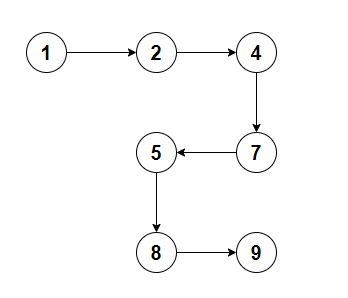
\includegraphics[width=\linewidth]{probelam2.1incisocfiguraa.jpg}
            \caption{figura a) 6 arcos}
            \label{fig:figura1}
            \end{minipage}
            \hspace{0.5cm}
            \begin{minipage}[b]{0.4\linewidth}
            \centering
            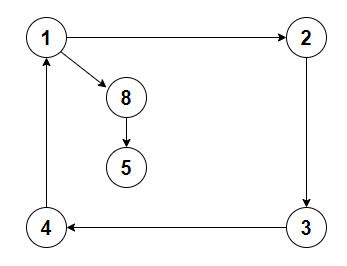
\includegraphics[width=\linewidth]{problema2.21incisocfigurab.jpg}
            \caption{figura b) 6 arcos}
            \label{fig:figura2}
            \end{minipage}
        \end{figure}
        \begin{figure}[ht]
            \begin{minipage}[b]{0.4\linewidth}
            \centering
            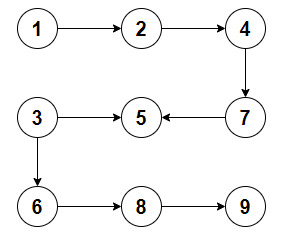
\includegraphics[width=\linewidth]{2.1incisoc8arcosfiguraa.jpeg}
            \caption{figura a) 8 arcos}
            \label{8 arcos 1}
            \end{minipage}
            \hspace{0.5cm}
            \begin{minipage}[b]{0.4\linewidth}
            \centering
            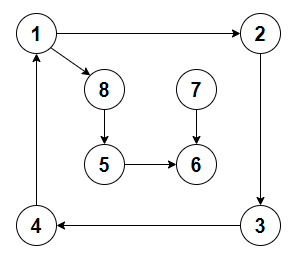
\includegraphics[width=\linewidth]{2.1incisoc8arcosfigurab.jpeg}
            \caption{figura b) 8 arcos}
            \label{8 arcos 2}
            \end{minipage}
        \end{figure}
        \newpage
        \item Specify a cycle containing nine arcs and a directed cycle containing seven arcs.
        \begin{figure}[h]
            \begin{minipage}[b]{0.4\linewidth}
            \centering
            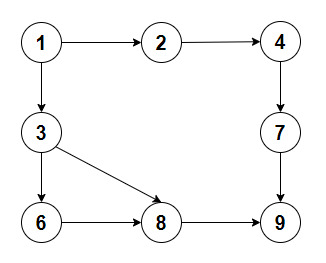
\includegraphics[scale = 0.5]{problema2.1incisodfigurab9arcos.jpeg}
            \caption{figura a) 9 arcos}
            \label{fig:figura3}
            \end{minipage}
            \hspace{0.5cm}
            \begin{minipage}[b]{0.4\linewidth}
            \centering
            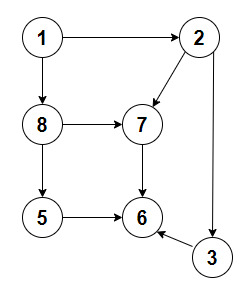
\includegraphics[scale = 0.5]{problema2.1incisodfiguraa9arcos.jpeg}
            \caption{figura b 9) arcos}
            \label{fig:figura4}
            \end{minipage}
        \end{figure}
        \begin{figure}[h]
            \centering
            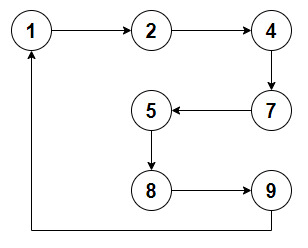
\includegraphics[scale = 0.5]{problema2.1incisodfiguraa7arcos.jpeg}
            \caption{figura a) 7 arcos}
        \end{figure}
    \end{enumerate} % fin del problema 2.1
    \item Specify a spanning tree of the graph in Figure 2.26(a) with six leaves. Specify a cut of
    the graph in Figure 2.26(a) containing six arcs.
    \begin{figure}[h]
        \centering
        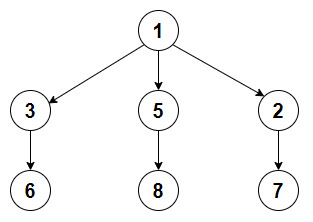
\includegraphics[scale = 0.5 ]{problema2.2arbol.jpeg} 
        \caption{figura 2.26 (a)}       
    \end{figure} 
    \newpage
     El corte será de $s = \{ 1,2,3,5,4 \}$ y $t = \{ 6,7,8,9 \}$ y se mostrarán en las siguientes figuras:
    \begin{figure}[h!]
        \begin{minipage}[b]{0.4\linewidth}
        \centering
        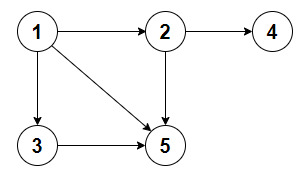
\includegraphics[width=\linewidth]{problema2.2corteparte1.jpeg}
        \caption{corte 1}
        \end{minipage}
        \hspace{0.5cm}
        \begin{minipage}[b]{0.4\linewidth}
        \centering
        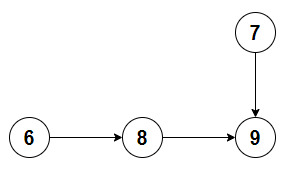
\includegraphics[width=\linewidth]{problema2.2corteparte2.jpeg}
        \caption{corte 2}
        \end{minipage}
    \end{figure} % final del problema 2.2

    \item For the graphs shown in Figure 2.26, answer the following questions.
    %incisos del problema 2.3
    \begin{enumerate}[(a)]
        \item Are the graphs acyclic?
        \\ Como se mostró en el ejercicio 2.21 inciso c) ambos grafos contienen un ciclo no dirigido, lo cual es la definición de acíclico.
        
        \item Are the graphs bipartite?
        \\ La figura a no es bipartite, mientras que la figura b si lo es, se mostrarán las siguientes imágenes:
        \begin{figure}[h]
            \begin{minipage}[b]{0.4\linewidth}
            \centering
            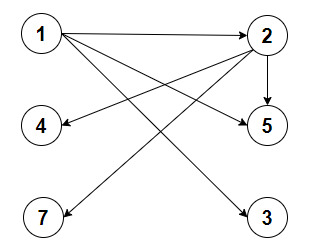
\includegraphics[scale = 0.5]{2.3incisobfiguraa.jpeg}
            \caption{Observe el arco (2,5)}
            \end{minipage}
            \hspace{0.5cm}
            \begin{minipage}[b]{0.4\linewidth}
            \centering
            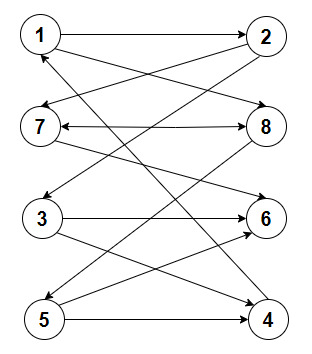
\includegraphics[scale = 0.5]{2.3incisobfigurab.jpeg}
            \caption{Se parte en dos subconjuntos}
            \end{minipage}
        \end{figure}
        \item Are the graphs strongly connected?
        \\ No, ya que ninguno de los dos grafos contiene un \textit{directed path}.
    \end{enumerate} % fin del problema 2.3
    \item Consider the graphs shown in Figure 2.26.
    %incisos del problema 2.24
    \begin{enumerate}[(a)]
        \item Do the graphs contain a directed in-tree for some root node?
        \begin{figure}[ht]
            \begin{minipage}[b]{0.4\linewidth}
            \centering
            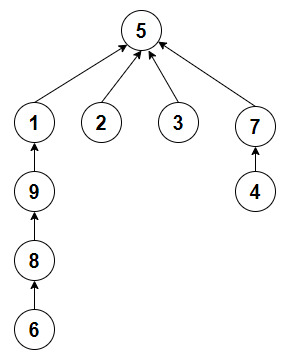
\includegraphics[scale = 0.5]{2.4incisoafiguraa.jpeg}
            \caption{in-tree figura a}
            \end{minipage}
            \hspace{0.5cm}
            \begin{minipage}[b]{0.4\linewidth}
            \centering
            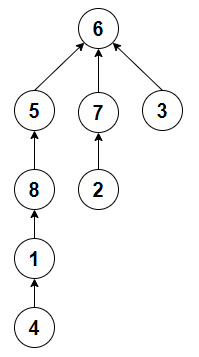
\includegraphics[scale = 0.5]{2.4incisoafigurab.jpeg}
            \caption{in-tree figura b}
            \end{minipage}
        \end{figure}
        \newpage
        \item Do the graphs contain a directed out-tree for some root node?
        \begin{figure}[ht]
                    \begin{minipage}[b]{0.4\linewidth}
                    \centering
                    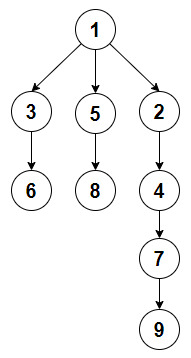
\includegraphics[scale = 0.5]{2.4incisobfiguraa.jpeg}
                    \caption{out-tree figura a}
                    \end{minipage}
                    \hspace{0.5cm}
                    \begin{minipage}[b]{0.4\linewidth}
                    \centering
                    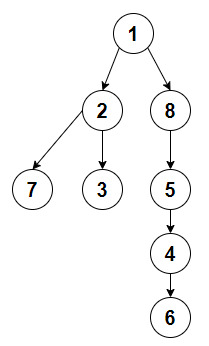
\includegraphics[scale = 0.5]{2.4incisobfigurab.jpeg}
                    \caption{out-tree figura b}
                    \end{minipage}
                \end{figure}
        \item In Figure 2.26(a), list all fundamental cycles with respect to the following spanning
        tree $T = {(1, 5), (1, 3), (2, 5), (4, 7), (7, 5), (7, 9), (5, 8), (6, 8)}$.
        \begin{table}[h!t] %tabla de ciclos
            \centering
            \resizebox*{4 cm}{!}{\begin{tabular}{|c|c|}
                \hline
                \textbf{arc} & \textbf{cycle}     \\ \hline
                (1,2)         & \textit{1-2-5-1}   \\ \hline
                (2,4)         & \textit{2-4-7-5-2} \\ \hline
                (2,7)         & 2-7-5-2            \\ \hline
                (3,6)         & 3-6-8-5-1-3        \\ \hline
                (3,5)         & 3-5-1-3            \\ \hline
                (3,8)         & 3-8-5-1-3          \\ \hline
                (5,9)         & 5-9-7-5            \\ \hline
                (8,9)         & 8-9-7-5-8          \\ \hline
                (9,1)         & 9-1-5-7-9          \\ \hline
                \end{tabular}}
            \end{table}
        \newpage
        \item For the spanning tree given in part (c), list all fundamental cuts. Which of these
        are the s-t cuts when s = 1 and t = 9?
        \begin{table}[ht]
            \centering
            \begin{tabular}{|l|l|l|l|l|l|l|l|l|}
            \hline
            \textbf{elemental cut} & \textit{(1,3)} & \textit{(1,5)} & \textit{(2,5)} & \textit{(4,7)} & \textit{(5,8)} & \textit{(6,8)} & \textit{(7,5)} & \textit{(7,9)} \\ \hline
            \end{tabular}
            \end{table} \newline
        Los únicos cortes que son  s-t con esas características son: $(7,9), (7,5), (1,5)$
    \end{enumerate} % fin de los incisos problema 2.4
   
    \item  Construct:
    \begin{enumerate}[(a)]
        \item Construct a directed strongly connected graph with five nodes and five arcs.
        \begin{figure}[h!t]
            \centering
            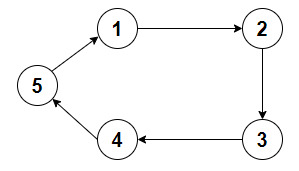
\includegraphics[scale = 0.5]{2.5incisoa.jpeg}
            \caption{strongly connected}
        \end{figure}
        \item Construct a directed bipartite graph with six nodes and nine arcs.
        \begin{figure}[h!t]
            \centering
            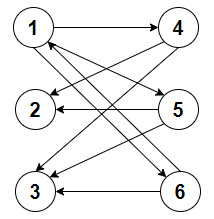
\includegraphics[scale = 0.5]{2.5incisob.jpeg}
            \caption{Bipartite}
        \end{figure}
        \item Construct an acyclic directed graph with five nodes and ten arcs.
        \begin{figure}[h!t]
            \centering
            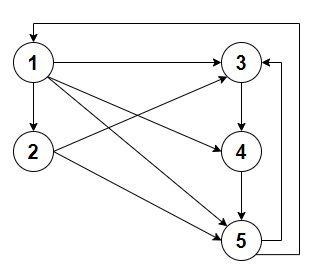
\includegraphics[scale = 0.5]{2.5incisoc.jpeg}            
        \end{figure}
    \end{enumerate} % final de los incisos problema 2.5
    \newpage
    \item {\bfseries Bridges of Konigsberg}. The first paper on graph theory was written by Leonhard Euler
    in 1736. In this paper, he started with the following mathematical puzzle: The city of
    Konigsburg has seven bridges, arranged as shown in Figure 2.27. Is it possible to start
    at some place in the city, cross every bridge exactly once, and return to the starting
    place? Either specify such a tour or prove that it is impossible to do so.
    \\ Para responder este problemas enunciaremos el siguiente teorema:
    \begin{theo}{}{}
        Sea G un grafo o multigrafo no dirigido. Entonces G tiene un ciclo de Euler si, y solo si, es conexo y todo vértice tiene grado par. Diremos que es un grafo Euleriano
    \end{theo}
    Veamos la siguiente imagen:
    \begin{figure}[ht]
        \centering
        \includegraphics[scale = 0.4]{puente de königsberg.png}
        \label{puente}
    \end{figure}
    \\ Si observamos la figura 2.27 en ella se marcaron unos puntos, los cuales haremos nodos para dibujar la siguiente red:
    \begin{figure}[ht]
        \centering
        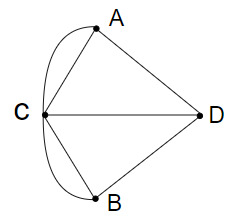
\includegraphics[scale = 0.5]{diagrama puente.jpeg}
    \end{figure}
    \newpage La red anterior es una red conexa no dirigida; obtengamos el grado de cada vértice:
    \begin{table}[ht]
        \centering
        \begin{tabular}{|c|c|}
        \hline
        \textbf{vértice} & \textbf{grado} \\ \hline
        \textbf{A}       & \textit{3}     \\ \hline
        \textbf{B}       & \textit{3}     \\ \hline
        \textbf{C}       & \textit{5}     \\ \hline
        \textbf{D}       & \textit{3}              \\ \hline
        \end{tabular}
    \end{table}
    \\ Como podemos observar todos son impares entonces no existe un ciclo de euler, por lo cual no podemos lograr pasar por todos los puentes una sola vez.
    \\ Existe un corolario de la siguiente manera:
    \begin{tcolorbox}[colback=black!5!white,colframe=black!80!white,title=Corolario 1:]
        Si G es un grafo o multigrafo no dirigido, se puede construir un camino de euler de G si y solo si G es conexo y tiene sólo dos vértices de grado impar.
    \end{tcolorbox}
    En este caso tampoco se satisface. % final del problema 2.6
    \item[2.22] The k-color problem on an undirected graph $G = (N, A)$ is defined as follows: Color
    all the nodes in N using at most $k$ colors so that for every arc $(i, j) \in A$, nodes $i$ and
    $j$ have a different color.
    \begin{enumerate}[(a)]
        \item Given a world map, we want to color countries using at most k colors so that the
        countries having common boundaries have a different color. Show how to formulate
        this problem as a k-color problem.
        \\ Sea $G = (V,E)$ un grado no dirigido, dividiremos el conjunto de vértices $V$ en $k$ subconjuntos con las siguientes propiedas:
        \begin{equation} \label{disjuntos}
            V_i \cap V_j \neq \emptyset, \hspace{0.5 in } \forall i \neq j  
        \end{equation}
        \begin{equation} \label{union}
            \bigcup_{j=1}^ {k} V_j = V
        \end{equation}
        En la ecuación \ref{disjuntos} evita superposición, mientras que en la ecuación \ref{union} queremos que la unión sea igual a todos los vértices.
        \\ Cada $V_i$ será llamado clase de color, si todos los vértices en una clase de color forman un conjunto estable\footnote{Ninguno de sus vértices es adyacente a otro} entonces será llamado \textit{k-colorante}. \\
        Para poder formular el problema tendremos que poner una cota superior:  $k_{\text{max}}$ de tal manera que el número óptimo de colores $k$ es un entero tal que $1 \leq k \leq k_{\text{max}}$ .
        \\ Definiremos una variable binaria $x_{ik}$ talque cuando el vértice $i$ sea asignado al color $k$ tomará el valor de 1 y 0 en otro caso. Además otra variable binaria $y_k$ tal que se podrá usar el color $k$ solo si $y_k = 1$ 
        \\ Veamos el modelo:
        \begin{align}
            \label{objetivo} \text{Minimizar: } \hspace{0.2 in} & \sum_{k=1}^{k_{\text{max}}} y_k \\
            \label{rest1} \text{Sujeto a: } \hspace{0.2 in}  & \sum_{k=1}^{k_{\text{max}}} x_{ik} = 1 \hspace{0.2 in} \forall i \in V  \\
            \label{rest2} & x_{ik} + x_{jk} \leq y_k \hspace{0.1 in} \forall \{i,j\} \in E;k=1, \cdots, k_{\text{max}} \\
            \label{rest3} & x_{ik} \in \{0,1\} \hspace{0.2 in} \forall i \in V;k=1, \cdots, k_{\text{max}} \\
            \label{rest4} & y_{k} \in \{0,1\} \hspace{0.2 in } k=1, \cdots, k_{\text{max}}
        \end{align}
        En la primer restricción con índice \ref{rest1} se garantiza que exactamente un color sea asignado a cada vértice. En la segunda restricción con índice \ref{rest2} tenemos una relación entre las variables $x$ y $y$ de tal manera que evita que vértices $i$ y $j$ tengan el mismo color simultáneamente.
        \\ En los índices \ref{rest3} y \ref{rest4} definimos la naturaleza de las variables.
        \item Show that a graph is bipartite if and only if it is 2-colorable (i.e., can be colored
        using at most two colors).
        \\ Supongamos que tenemos un grafo bipartito, entonces podemos hacer la igualdad de $V= V_1 \cup V_2$ de tal manera que todos los vértices en $V_1$ son disjuntos, lo mismo para $V_2$ lo cual es la definición de \textit{k-colorante}, por lo cual tenemos dos colores.
        \\ Ahora supongamos que solo tenemos dos colores para pintar esto nos deja las ecuaciones de la siguiente manera:
        \begin{align*}
             \text{Minimizar: } \hspace{0.2 in} & y_1+y_2 \\
             \text{Sujeto a: } \hspace{0.2 in}  &  x_{i1} + x_{i2} = 1 \hspace{0.2 in}  \forall i \in V \\
             & x_{i1} + x_{j1} \leq y_1 \hspace{0.1 in} \forall \{i,j\} \in E\\
             & x_{i2} + x_{j2} \leq y_2 \hspace{0.1 in} \forall \{i,j\} \in E\\
             & x_{ik} \in \{0,1\} \hspace{0.2 in} \forall i \in V;k=1, \cdots, k_{\text{max}} \\
             & y_{k} \in \{0,1\} \hspace{0.2 in } k=1, \cdots, k_{\text{max}}
        \end{align*}
        Si observamos las ecuaciones anteriores, podemos decir que si el nodo tine asignado el color $k=1$ todos los nodos adyacentes tendrán que ser de color $k= 2$, ahora si recordamos la definición de grafo Bipartito tenemos dos conjuntos talque ambos tienen todos sus vértices disjuntos, lo cual satisface lo anterior.
    %final del problema 2.22
    \end{enumerate} \newpage
    \item[2.30] Specify the node-arc incidence matrix and the node-node adjacency matrix for
    the graph shown in Figure 2.28.
    \begin{figure}[ht]
        \centering
        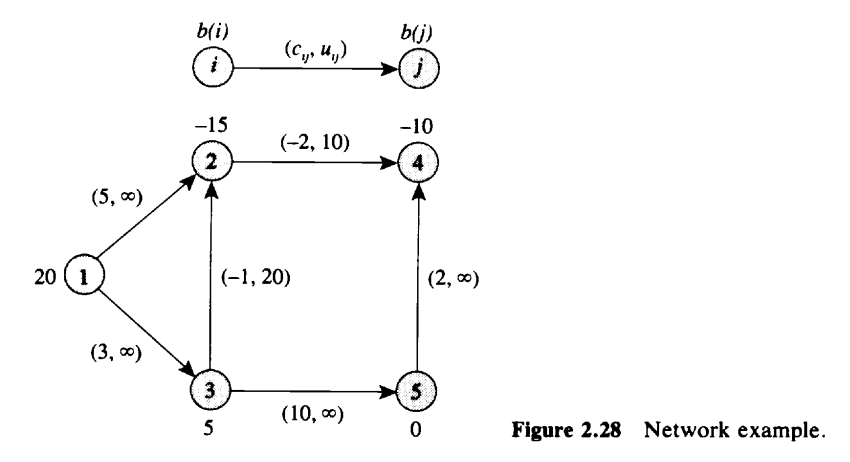
\includegraphics[scale = 0.3]{2.30.png}
    \end{figure}
    \begin{table}[ht]
        \centering
        \begin{tabular}{|ccccccc|}
        \hline
        \multicolumn{7}{|c|}{\textbf{node-arc}}                                                                                                                                                                                                         \\ \hline
        \multicolumn{1}{|c|}{}           & \multicolumn{1}{c|}{\textbf{(1,2)}} & \multicolumn{1}{c|}{\textbf{(1,3)}} & \multicolumn{1}{c|}{\textbf{(3,2)}} & \multicolumn{1}{c|}{\textbf{(2,4)}} & \multicolumn{1}{c|}{\textbf{(3,5)}} & \textbf{(5,4)} \\ \hline
        \multicolumn{1}{|c|}{\textbf{1}} & \multicolumn{1}{c|}{1}              & \multicolumn{1}{c|}{1}              & \multicolumn{1}{c|}{0}              & \multicolumn{1}{c|}{0}              & \multicolumn{1}{c|}{0}              & 0              \\ \hline
        \multicolumn{1}{|c|}{\textbf{2}} & \multicolumn{1}{c|}{-1}             & \multicolumn{1}{c|}{0}              & \multicolumn{1}{c|}{-1}             & \multicolumn{1}{c|}{1}              & \multicolumn{1}{c|}{0}              & 0              \\ \hline
        \multicolumn{1}{|c|}{\textbf{3}} & \multicolumn{1}{c|}{0}              & \multicolumn{1}{c|}{-1}             & \multicolumn{1}{c|}{1}              & \multicolumn{1}{c|}{0}              & \multicolumn{1}{c|}{1}              & 0              \\ \hline
        \multicolumn{1}{|c|}{\textbf{4}} & \multicolumn{1}{c|}{0}              & \multicolumn{1}{c|}{0}              & \multicolumn{1}{c|}{0}              & \multicolumn{1}{c|}{-1}             & \multicolumn{1}{c|}{0}              & -1             \\ \hline
        \multicolumn{1}{|c|}{\textbf{5}} & \multicolumn{1}{c|}{0}              & \multicolumn{1}{c|}{0}              & \multicolumn{1}{c|}{0}              & \multicolumn{1}{c|}{0}              & \multicolumn{1}{c|}{-1}             & 1              \\ \hline
        \end{tabular}
        \end{table}
        \begin{table}[ht]
            \centering
            \begin{tabular}{|llllll|}
            \hline
            \multicolumn{6}{|c|}{\textbf{Node-node}}                                                                                                                                                       \\ \hline
            \multicolumn{1}{|l|}{}           & \multicolumn{1}{l|}{\textit{\textbf{1}}} & \multicolumn{1}{l|}{\textbf{2}} & \multicolumn{1}{l|}{\textbf{3}} & \multicolumn{1}{l|}{\textbf{4}} & \textbf{5} \\ \hline
            \multicolumn{1}{|l|}{\textbf{1}} & \multicolumn{1}{l|}{\textit{0}}                   & \multicolumn{1}{l|}{\textit{1}} & \multicolumn{1}{l|}{\textit{1}} & \multicolumn{1}{l|}{\textit{0}} & \textit{0} \\ \hline
            \multicolumn{1}{|l|}{\textbf{2}} & \multicolumn{1}{l|}{\textit{0}}                   & \multicolumn{1}{l|}{\textit{0}} & \multicolumn{1}{l|}{\textit{0}} & \multicolumn{1}{l|}{\textit{1}} & \textit{0} \\ \hline
            \multicolumn{1}{|l|}{\textbf{3}} & \multicolumn{1}{l|}{\textit{0}}          & \multicolumn{1}{l|}{\textit{1}} & \multicolumn{1}{l|}{\textit{0}} & \multicolumn{1}{l|}{\textit{0}} & \textit{1} \\ \hline
            \multicolumn{1}{|l|}{\textbf{4}} & \multicolumn{1}{l|}{\textit{0}}          & \multicolumn{1}{l|}{\textit{0}} & \multicolumn{1}{l|}{\textit{0}} & \multicolumn{1}{l|}{\textit{0}} & \textit{0} \\ \hline
            \multicolumn{1}{|l|}{\textbf{5}} & \multicolumn{1}{l|}{\textit{0}}          & \multicolumn{1}{l|}{\textit{0}} & \multicolumn{1}{l|}{\textit{0}} & \multicolumn{1}{l|}{\textit{1}} & \textit{0} \\ \hline
            \end{tabular}
            \end{table}
    \item[2.42] Consider the minimum cost flow problem shown in Figure 2.28. Suppose that arcs
    $(1, 2)$ and $(3, 5)$ have lower bounds equal to $l_{12} = l_{35} = 5$. Transform this problem to
    one where all arcs have zero lower bounds
    \begin{figure}[h!t]
                \begin{minipage}[b]{0.4\linewidth}
                \centering
                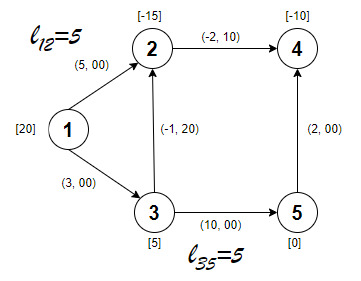
\includegraphics[scale = 0.5]{2.42 parte1.jpeg}
                \caption{Con limites inferiores.}
                \end{minipage}
                \hspace{0.5cm}
                \begin{minipage}[b]{0.4\linewidth}
                \centering
                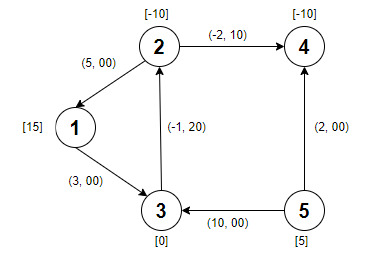
\includegraphics[scale = 0.5]{2.42 parte2.jpeg}
                \caption{Sin limites inferiores.}
                \end{minipage}
            \end{figure}
\end{enumerate}

\end{document}